\documentclass{beamer}

\usepackage{graphicx}
\usepackage{listings}
\usepackage[utf8]{inputenc}
\usepackage{tikz}
\usetikzlibrary {intersections, graphs, calc}


%30 min

\lstset{
  basicstyle=\footnotesize,        % the size of the fonts that are used for the code
  breakatwhitespace=true,          % sets if automatic breaks should only happen at whitespace
  breaklines=true,                 % sets automatic line breaking
  commentstyle=\color{green},      % comment style
  keywordstyle=\color{blue},       % keyword style
  language=C++,                    % the language of the code
  numbers=none,                    % where to put the line-numbers; possible values are (none, left, right)
}


\newcommand{\sectiontitle}[1]{
    \section{#1}
    \begin{frame}
        \centering
        \Huge{#1}
    \end{frame}
}
\newcommand{\subsectiontitle}[1]{
    \subsection{#1}
    \begin{frame}
        \LARGE{#1}
    \end{frame}
}

\newcommand{\inlinecpp}[1]{
    \lstinline[language=C++]{#1}
}


\title[ugtest]{ugtest}
\author{Tobias Trautmann}
\institute{GCSC}

\begin{document}

    \begin{frame}
        \titlepage
    \end{frame}

    \begin{frame}{Outline}
        \tableofcontents
    \end{frame}

    \sectiontitle{Introduction to testing}
        % Vertrauen ins testsystem? z.B. Review (Review Kriterien, Methoden)? Studenten untereinander codereview?
        \subsection{Goals}
        \begin{frame}{Goals of testing}
            %nur geteste software erzeugt wert
            %it := Software
           \begin{itemize}
                \item increase trust in its results\pause
                \item make code maintainable\pause
                \item make code refactorable\pause
                \item make it sufficiently robust\pause
                \item check if it performs its functions within an acceptable time\pause
                \item check wether in runs its intended environments\pause
           \end{itemize}
           \Large{$\Rightarrow$ Testing software is a \textbf{necessity}}
        \end{frame}

        \subsection{Defects}
        \begin{frame}{Defects}
            Where do defects come from?\\
            \begin{itemize}
                \item error in design
                \item bug in code
                \item script error (lua)
                \item integration
            \end{itemize}
            $\Rightarrow$ Makes clear what to test with which priority

        \end{frame}
        
        \subsection{Test Pyramid}
        \begin{frame}[plain]{Test Pyramid}
            %Talk about each test level, what it does what its for and when to do them
            % pesticide paradox\\%bugs become more subtle the more you cover
            % testen für qualität nicht für statistik!!
            % amount of work put into testing 25\%-50\% of total  time!!!!!
            % entwicklungsbegleitendes testen
            \centering
            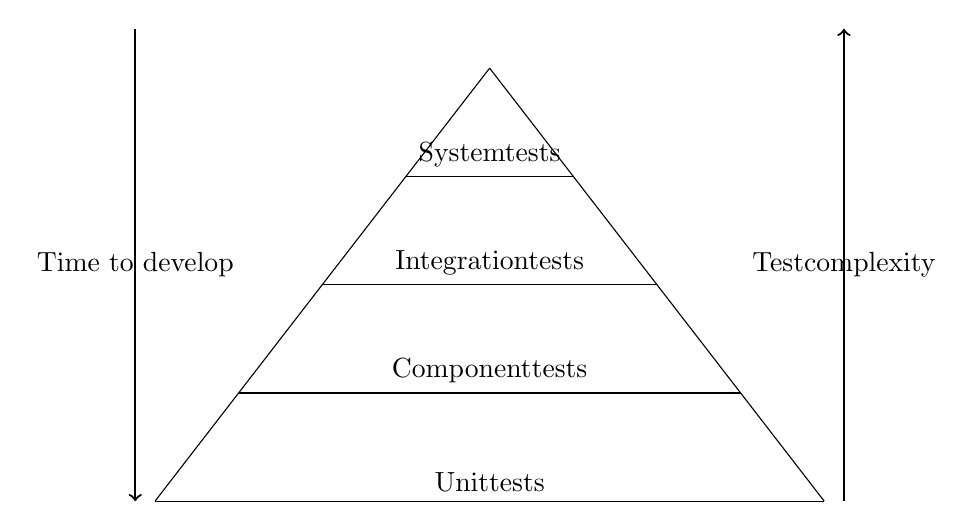
\begin{tikzpicture}
                \coordinate (A) at (-4.25,-1) {};
                \coordinate (B) at ( 4.25,-1) {};
                \coordinate (C) at (0,4.5) {};
                \draw[name path=AC] (A) -- (C);
                \draw[name path=BC] (B) -- (C);
                \draw[name path=AB] (A) -- (B);
    
                \foreach \y/\A in {0/Unittests,1/Componenttests, 2/Integrationtests, 3/Systemtests} {
                    \draw ($(A)!\y/4!(C)$) -- ($(B)!\y/4!(C)$) node[midway,above] {\A};\pause
                }
                \draw[thick, ->] (-4.5,5) -- (-4.5, -1) node[midway] {Time to develop};\pause
                \draw[thick, <-] (4.5,5) -- (4.5, -1) node[midway] {Testcomplexity};
            \end{tikzpicture}
        \end{frame}

    \sectiontitle{Boost.Test}

        \subsection{Basic usage}
        \begin{frame}{Structure}
            \lstinputlisting[language=c++]{scripts/structure.cpp}
        \end{frame}

        \begin{frame}{Assertion Levels}
            \begin{tabular}{c|c|c}
                assertion level &   error counter   &   test case continuation   \\
                \hline
                warn    &       &   yes \\
                check   &   ++  &   yes \\
                require &   ++  &   no  \\
            \end{tabular}
        \end{frame}

        \begin{frame}{Basics}
            \begin{itemize}
                \item  \inlinecpp{BOOST_<level>(predicate)}
                \item  \inlinecpp{BOOST_<level>_<GE,LE,GT,LT,NE>(left, right)}
                \item  \inlinecpp{BOOST_<level>_EQUAL(left, right)}
                \item  \inlinecpp{BOOST_IS_DEFINED(SYMBOL)}
                \item  \inlinecpp{BOOST_<level>_MESSAGE(msg)}
            \end{itemize}
        \end{frame}

        \begin{frame}{Nice to know}
            \lstinputlisting[language=c++]{scripts/nice2know.cpp}
        \end{frame}

        \begin{frame}{Floating point comparison}
            \lstinputlisting[language=c++]{scripts/floatpoint_comparison.cpp}
        \end{frame}

        \begin{frame}{Exception handling}
            \lstinputlisting[language=c++]{scripts/exception_handling.cpp}      
        \end{frame}

        \subsection{Fixtures}
        \begin{frame}[plain]{Fixtures}
            \lstinputlisting[language=C++]{scripts/fixtures.cpp}
        \end{frame}

        \subsection{Templates}
        \begin{frame}[plain]{Templates}
            \lstinputlisting[language=C++]{scripts/templates.cpp}
        \end{frame}

    \sectiontitle{Testing}
        \subsection{Test executable}
        \begin{frame}{Test execution}
            \begin{itemize}
                \item add buildflags "-fprofile-arcs -ftest-coverage -fPIC" as well as no optimization for code coverage analysis
                \item build ug with UGTest and your plugin activated
                \item your plugin contains tests in a top level folder named "tests"
                %\item Your tests include UGTest.h
                \item executable named "ugtest\_unit" lands in ug4/bin
                \item example: \lstinline[language=bash]{ug4/bin $ ./ugtest_unit --log-level=ALL --log-format=HRF}
                % Show result
            \end{itemize}
        \end{frame}
        
        \subsectiontitle{Jenkins}

    \sectiontitle{Additional}
    %short
    \begin{frame}{Continous Integration / Continous Delivery}
        \centering
        \begin{figure}
            \includegraphics[width=12cm]{./images/cicd.jpeg}
        \end{figure}
    \end{frame}

    \begin{frame}[plain]{Git branching \& releases}
        \centering
        \begin{figure}
            \includegraphics[width=12cm]{images/branching.pdf} 
        \end{figure}
        sauce
    \end{frame}
   
    %short
    \begin{frame}{Test driven development}
        \centering
        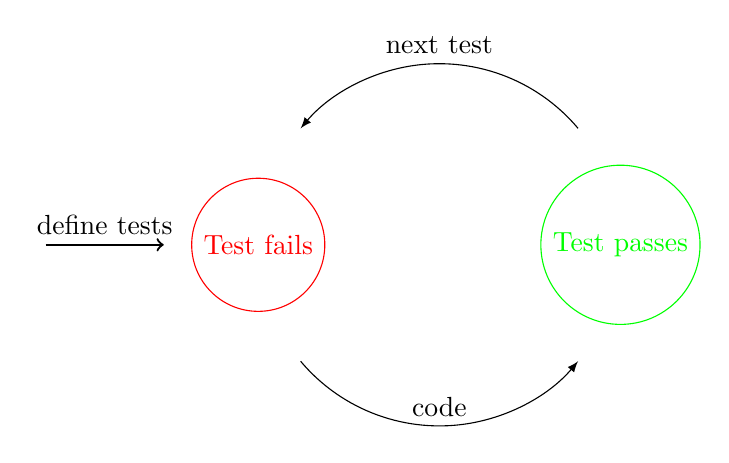
\begin{tikzpicture}
            \def \n {2}
            \def \radius {2.3cm}
            \def \margin {40}
            \draw[->,thick] (-5,0) -- (-3.5,0) node[midway, above] {define tests};
            \foreach \s/\A/\C/\N in {1/Test passes/green/next test,2/Test fails/red/code}
            {
                \node[draw, circle,\C] at ({360/\n * (\s - 1)}:\radius) {\A};
                \draw[->, >=latex] ({360/\n * (\s - 1)+\margin}:\radius) arc ({360/\n * (\s - 1)+\margin}:{360/\n * (\s)-\margin}:\radius) node[midway, above] {\N};
            }
        \end{tikzpicture}
    \end{frame}

    \begin{frame}{Toolchain}
        \begin{itemize}
            \item bugtracking
            \item documentation user / developer (Doxygen)
            \item \href{https://www.jenkins.io/doc/}{Jenkins}
            \item \href{https://www.gcovr.com/en/stable/guide.html}{gcovr (Code Coverage tool)}
            \item git storage
            \item \href{https://docs.docker.com/}{Docker}
            \item update boost?
            \item gcc + clang?
            \item Anforderung nacherfassen!! Danach Tolls richten
            \item wie requiremetns testen?
        \end{itemize}
    \end{frame}

    \begin{frame}{Standardization}
        \begin{itemize}
            \item definiton of done
            \item design for testability
            \item test structure
            \item naming conventions
        \end{itemize}
    \end{frame}

    \begin{frame}{Advanced}
        \begin{itemize}
            \item test data%possible within boost see data-driven test cases
            \item mocking
        \end{itemize}
    \end{frame}
    
    \begin{frame}{Additional resources}
            \begin{itemize}
                \item \href{https://www.boost.org/doc/libs/1_58_0/libs/test/doc/html/utf/user-guide/runtime-config/reference.html}{Boost.Test executable list of params}
                \item \href{https://www.boost.org/doc/libs/1_73_0/libs/test/}{newest Boost.Test} %(often better documentation of already existing features)
                \item \href{https://github.com/UG4/plugin_UGTest}{ugtests github}
                %\item \href{https://www.dreckstool.de}{dreckstools}
                \item \href{https://www.jenkins.io/doc/book/pipeline/syntax/}{Jenkins Pipeline}
                \item \href{https://martinfowler.com/articles/practical-test-pyramid.html}{Martin Fowler}
                \item \href{https://en.wikipedia.org/wiki/SOLID}{SOLID principle}
                \item \href{https://www.jenkins.io/doc/}{Jenkins docs}
            \end{itemize}
    \end{frame}

    \section{References}
    \begin{frame}{References}
        \begin{itemize}
            \item \href{https://en.wikipedia.org/wiki/Software_testing}{Wikipedi Softwaretests}
            \item \href{https://www.boost.org/doc/libs/1_58_0/libs/test/}{Boost.Test 1.58 documentation}
            %definitly wrong pls fix
            \item Basiswissen Softwaretest
            \item \href{https://docs.microsoft.com/en-us/azure/devops/repos/git/git-branching-guidance?view=azure-devops}{Microsoft branching}
        \end{itemize}
    \end{frame}
\end{document}